\documentclass[a4paper]{ctexart}

\usepackage{amsmath}
\usepackage{amssymb}
\usepackage[UTF8, scheme=plain]{ctex}
\usepackage{enumitem}
\usepackage{fancyhdr}
\usepackage{gensymb}
\usepackage[margin=1in]{geometry}
\usepackage{graphicx}  % 用于插入图片
\usepackage{hyperref}
\usepackage{indentfirst} % 首行缩进
\usepackage{lastpage}
\usepackage{ragged2e}
\usepackage{tikz}
\usepackage{upgreek}
\usepackage{verbatim}
\usepackage{xassoccnt}
\usepackage{wasysym} % 允许包含图像
\usepackage{chngcntr}
\usepackage{float}

\counterwithin*{enumi}{section} 

\usetikzlibrary{calc}

\date{} % not display time here

\fancyhf{}
\pagestyle{fancy} %fancyhdr宏包新增的页面风格

% foot decorative lines
\renewcommand{\footrulewidth}{1pt}
\fancyhead[R]{\leftmark}

\newcommand{\myoverline}[1]{%
  \leavevmode % 确保在段落中正常工作
  \rlap{\raisebox{2ex}{\rule{1.5cm}{0.4pt}}}% 上划线(位置0.5ex,粗细0.4pt)
  #1% 文本内容
}

\setmainfont{SimHei}

\begin{document}
    % whether show solutions 
    \newif\ifshowSolution
    % \showSolutiontrue
    \showSolutionfalse

    % 不显示自动编号 且 能自动生成目录
    \setcounter{secnumdepth}{0}
    % 行距
    \renewcommand{\baselinestretch}{1.25}

    \title{\heiti\zihao{2} 2025年迎春杯(小中)数学讲义}
    \maketitle
    \thispagestyle{empty} % 标题页不显示页码

    \vfill
    \centerline{\date{\today}}

    \setlength{\parindent}{2em}
    \newpage

    % 目录 罗马数字页码
    \setcounter{page}{1}
    \pagenumbering{Roman}
    \cfoot{\thepage}

    \hypersetup{colorlinks=true, linktocpage=true}
    \tableofcontents

    % 正文 阿拉伯数字页码
    \newpage
    \setcounter{page}{1}
    \pagenumbering{arabic}
    % 当前页 of 总页数
    \cfoot{\thepage\ / \pageref{LastPage}}

    \zihao{5}

    \begin{sloppy}
        \begin{enumerate}
            \section{第1讲\quad 计算}

\item {
    【乘法分配律】
    $(200+2)\times 5 + 5020$ 
    \ifshowSolution
        \fangsong\zihao{4}
        \\
        思路:改。2025

        正解: 
    \else
        \\ \\ \\
    \fi
}

% \item {
%     $(20+2)\times 5 + 2025$ 
%     \ifshowSolution
%         \fangsong\zihao{4}
%         \\
%         思路:2025

%         正解: 
%     \else
%         \\ \\ \\
%     \fi
% }

\item {
    【乘法分配律】
    $7\times 19 + 3\times 13\times 41 + 13\times 19$
    \ifshowSolution
        \fangsong\zihao{4}
        \\
        思路:改。2021;迎春杯四年级真题.pdf

        正解: 
    \else
        \\ \\ \\
    \fi
}

\item {
    【乘法分配律】
    $(18\times 23 - 24\times 17)\div 3 + 5$
    \ifshowSolution
        \fangsong\zihao{4}
        \\
        思路:

        正解: 
    \else
        \\ \\ \\
    \fi
}

\item {
    【乘法分配律】
    $(11\times 24 - 23\times 9)\div 3 + 3$
    \ifshowSolution
        \fangsong\zihao{4}
        \\
        思路:

        正解: 
    \else
        \\ \\ \\
    \fi
}

% \item {
%     【乘法分配律】
%     $7\times 17 + 3\times 13\times 43 + 13\times 17$
%     \ifshowSolution
%         \fangsong\zihao{4}
%         \\
%         思路:2021;迎春杯四年级真题.pdf

%         正解: 2017
%     \else
%         \\ \\ \\
%     \fi
% }

% \item {
%     $(9\times 8\times 7 + 6 - 5)\times 4 + 3 -2 +1$
%     \ifshowSolution
%         \fangsong\zihao{4}
%         \\
%         思路: 迎春杯四年级2022-试卷.pdf

%         正解: 2022
%     \else
%         \\ \\ \\
%     \fi
% }

\item {
    【乘法凑10】
    $12\times 25 + 16\times 15$
    \ifshowSolution
        \fangsong\zihao{4}
        \\
        思路:

        正解: 
    \else
        \\ \\ \\
    \fi
}

\item {
    【乘法凑10】
    $5\times 432\times 1 - 98 - 7\times 6$
    \ifshowSolution
        \fangsong\zihao{4}
        \\
        思路: 2020数学花园探秘笔试小中决赛D卷.doc

        正解: 2020
    \else
        \\ \\ \\
    \fi
}

\item {
    【加法凑10】
    $1+3+4+6+7+9+10 + 12$
    \ifshowSolution
        \fangsong\zihao{4}
        \\
        思路:

        正解: 
    \else
        \\ \\ \\
    \fi
}

\item {
    【乘法凑10】
    $210\times 6 - 52\times 5$
    \ifshowSolution
        \fangsong\zihao{4}
        \\
        思路:

        正解: 
    \else
        \\ \\ \\
    \fi
}

\item {
    【尾同头合十】
    $5000- 22\times 82$  
    \ifshowSolution
        \fangsong\zihao{4}
        \\
        思路:

        正解: 
    \else
        \\ \\ \\
    \fi
}

\item {
    【乘法分配律】
    $67\times 67 - 34\times 34 + 67 + 34$
    \ifshowSolution
        \fangsong\zihao{4}
        \\
        思路:2017年“迎春杯”数学花园探秘科普活动试卷(小中组决赛a卷).doc

        正解: 3434
    \else
        \\ \\ \\
    \fi
}

\item {
    【等差数列求和公式】
    $(1+3+5+\cdots + 89) - (1+2+3+\cdots + 63)$  
    \ifshowSolution
        \fangsong\zihao{4}
        \\
        思路:

        正解: 
    \else
        \\ \\ \\
    \fi
}

\item {
    【数列】
    数列$1, 1,2,3,5,8\cdots$从第二项起每一项都等于它前面两项之和,这个数列成为斐波那契数列.其中每一项都叫做斐波那契数.可以证明“任意正整数n都可以成若干个不同的斐波那契数之和”,那么把100表示成若干个不同的斐波那契数之和有\underline{\hbox to 20mm{}}种表示方法.(只是交换加数的顺序算作同一种)  
    \ifshowSolution
        \fangsong\zihao{4}
        \\
        思路: 2016年“迎春杯”数学花园探秘初赛试卷(四年级b卷).doc

        正解: 9
    \else
        \\ \\ \\
    \fi
}

\item {
    【立方和公式】
    $3^3 + 4^3 + 5^3 + 6^3 + 7^3 + 8^3 + 9^3$
    \ifshowSolution
        \fangsong\zihao{4}
        \\
        思路:

        正解: 
    \else
        \\ \\ \\
    \fi
}

\item {
    【数值计算】
    $99\times 10101\times 111\times 1001001$的末5位数字是多少?
    \ifshowSolution
        \fangsong\zihao{4}
        \\
        思路:

        正解: 88889
    \else
        \\ \\ \\
    \fi
}

\item {
    【数值计算;数字谜】
    正着读和反着读都一样的数称为回文数,如121、9889都是回文数,如果一个三位回文数和一个四位回文数的和是 2025,那么这两个回文数的差是\underline{\hbox to 20mm{}}.
    \ifshowSolution
        \fangsong\zihao{4}
        \\
        思路: 综合-数字谜.

        正解: 改  2023;YCB第40届小中组试卷.pdf; 1551+474=2025
    \else
        \\ \\ \\
    \fi
}

\item {
    【数值计算;数字谜】有一些自然数,如 121 和 2552,从左到右和从右到左的数字顺序相同,我们把这样的自然数叫做``回文数''. 已知两个回文数的和是 2022,则这两个回文数的差是\underline{\hbox to 20mm{}}.
    \ifshowSolution
        \fangsong\zihao{4}
        \\
        思路: 综合-数字谜.

        正解:  迎春杯三年级2022-试卷.pdf; 1740
    \else
        \\ \\ \\
    \fi
}

% \item {
%     【数字谜】
%     下列竖式中,相同汉字表示相同数字,不同汉字表示不同数字,且所有汉字对应的数字都不是 0,2,5。 ``空歌风度清'' 表示的五位数是\underline{\hbox to 20mm{}}.
%     \zihao{2}
%     \begin{figure}[H] 
%         \centering
%         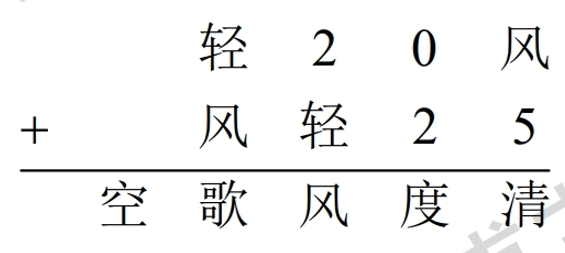
\includegraphics[width=0.4\textwidth]{./pics/Chapter_7/1.png}
%     \end{figure}
%     \vspace{1cm}
%     % 2025数学花园探秘笔试小中年级决赛C卷(B5试卷版).pdf;16934
% }

\item {
    【数字谜】
    下面的算式中,相同的汉字代表相同的数字,不同的汉字代表不同的数字,那么,\\ \myoverline{龙行天下}  表示的四位数是\underline{\hbox to 20mm{}}.
    \begin{figure}[H] 
        \centering
        
\includegraphics[width=0.4\textwidth]{./pics/Chapter_7/2.png}
    \end{figure}
    \vspace{1cm}
    % 2024
}

\item {
    【数字谜】
    将 $1\sim 9$分别填入到右图的方框中,每个数字用一次,使得竖式成立;现在数字 6、7、8已经被填入,那么竖式的和是\underline{\hbox to 20mm{}}.
    \zihao{2}
    \[
    \begin{array}{r@{\,}r@{}c@{}l}
    & \square & \square & \square \\
    + & \square  & \boxed{7} & \boxed{6} \\
    \cline{1-4}
    & \boxed{8} & \square & \square \\
    \end{array}
    \]
    % \begin{figure}[H] 
    %     \centering
    %     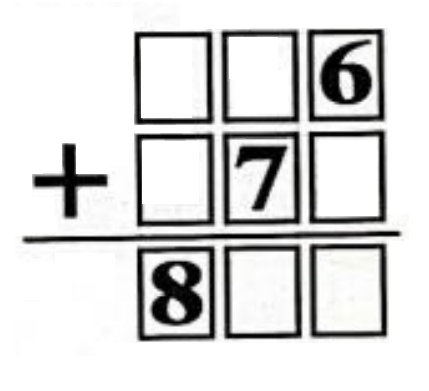
\includegraphics[width=0.3\textwidth]{./pics/Chapter_7/3.png}
    % \end{figure}
    \vspace{1cm}
    % 2023YCB初赛真题答案小中.pdf; 819
    % 改
}

\item {
    【数字谜】
    在右图的加法竖式中,6个汉字恰好代表6个连续的数字,那么,``花园探秘'' 所代表的四位数是\underline{\hbox to 20mm{}}.
    \begin{figure}[H] 
        \centering
        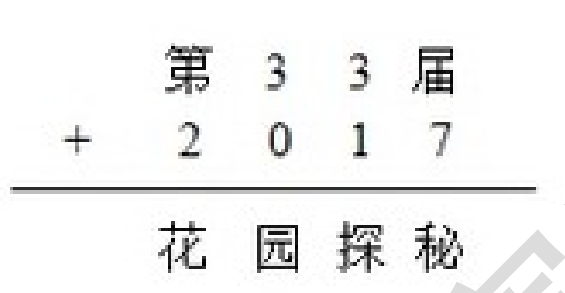
\includegraphics[width=0.4\textwidth]{./pics/Chapter_7/12.png}
    \end{figure}
    \vspace{1cm}
    % 2021; 8354
}

\item {
    【数字谜】
    在右面的乘法竖式中,相同的汉字代表相同的数字,不同的汉字代表不同的数字;那么,\myoverline{迎接夏天} 代表的四位数是\underline{\hbox to 20mm{}}.
    \begin{figure}[H] 
        \centering
        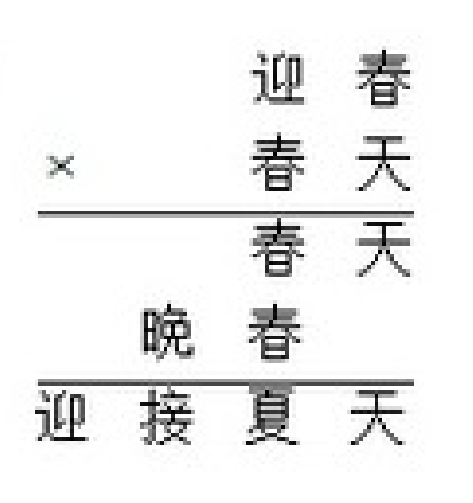
\includegraphics[width=0.4\textwidth]{./pics/Chapter_7/14.png}
    \end{figure}
    \vspace{1cm}
    % 2021,迎春杯四年级真题.pdf; 1024
}
        \end{enumerate}
        \begin{enumerate}
            \section{数论}

\title[第2讲\quad 数论]{第2讲\quad 数论} 
\author{}
\date{}

\begin{frame}
    \titlepage
\end{frame}

\setcounter{framecounter}{0}

\begin{frame}
    \stepcounter{framecounter}
    \frametitle{习题\theframecounter}
    \vspace*{-3cm}
    \center\textit{再过12天就到2016年了,昊昊感慨地说:我到目前只经过2个闰年,并且我出生的年份是9的倍数,那么2016年昊昊是 \underline{\hbox to 20mm{}} 岁.} 
    % 9
\end{frame}

\begin{frame}
    \stepcounter{framecounter}
    \frametitle{习题\theframecounter}
    \vspace*{-3cm}
    \textit{一个整数减去 77,然后乘以 8,再除以 7,所得的商是 37,而且有余数。这个数是多少?} 
    % 110
\end{frame}

\begin{frame}
    \stepcounter{framecounter}
    \frametitle{习题\theframecounter}
    \vspace*{-3cm}
    \textit{王老师在一个特殊的学校上课,他每上3天课可以休息一天,已知本学期他第一次休息在星期二,那么他第五次休息是星期\underline{\hbox to 20mm{}} (填数字1--7).} % 4
\end{frame}

\begin{frame}
    \stepcounter{framecounter}
    \frametitle{习题\theframecounter}
    \vspace*{-3cm}
    \textit{今天是1月30日,我们先写下130;后面写数的规则是:如果刚写下的数是偶数就把它除以2再加上2写在后面,如果刚写下的数是奇数就把它乘以2再减去2写在后面,于是得到:130、67、132、68…,那么这列数中第2016个数是\underline{\hbox to 20mm{}}} % 6
\end{frame}

\begin{frame}
    \stepcounter{framecounter}
    \frametitle{习题\theframecounter}
    \vspace*{-3cm}
    \textit{一组有两位数组成的偶数项等差数列,所有奇数项的和为100,若从第1项开始,将每个奇数项与它后面相邻的偶数项不改变次序地合并成一个四位数,形成一个新的数列,那么新数列的和与原数列的和相差\underline{\hbox to 20mm{}}.} % 9900
\end{frame}

\begin{frame}
    \stepcounter{framecounter}
    \frametitle{习题\theframecounter}
    \vspace*{-3cm}
    \textit{现在有一台奇怪的电脑,电脑上有个按键,如果电脑上原来的数是3的倍数,按下键后就会除以3;如果电脑上原来的数不是3的倍数,那么按下键后就会乘以6.小明在按键前没有看屏幕上的数,结果连按6次,最后电脑上显示的数是12,那么电脑上最开始的数最小可能是\underline{\hbox to 20mm{}}.} % 27
\end{frame}

\begin{frame}
    \stepcounter{framecounter}
    \frametitle{习题\theframecounter}
    \vspace*{-3cm}
    \textit{有一些自然数,如 121 和 2552,从左到右和从右到左的数字顺序相同,我们把这样的自然数叫做“回文数”.已知两个回文数的和是 2022,则这两个回文数的差是\underline{\hbox to 20mm{}}.} 
    % 2022; 
\end{frame}

\begin{frame}
    \stepcounter{framecounter}
    \frametitle{习题\theframecounter}
    \vspace*{-3cm}
    \textit{$99\times 10101\times 111\times 1001001$的末5位数字是多少?} % 88889
\end{frame}

\begin{frame}
    \stepcounter{framecounter}
    \frametitle{习题\theframecounter}
    \vspace*{-3cm}
    \textit{已知 $S = 2^{2020} + 3^{2021} + 4^{2022} + 5^{2023} +6^{2024} + 7^{2025}$, 则 $S$ 的末位数字是多少?} % 3
\end{frame}

\begin{frame}
    \stepcounter{framecounter}
    \frametitle{习题\theframecounter}
    \vspace*{-3cm}
    \textit{数列 $121, 1221, 12221, 122221,\cdots$ 的前2025项中,有多少项能被3整除?} % 675
\end{frame}

\begin{frame}
    \stepcounter{framecounter}
    \frametitle{习题\theframecounter}
    \vspace*{-3cm}
    \textit{有一个数除以3余 2,除以4余 1. 此数除以 12 余\underline{\hbox to 20mm{}}.} % 5
\end{frame}

\begin{frame}
    \stepcounter{framecounter}
    \frametitle{习题\theframecounter}
    \vspace*{-3cm}
    \textit{各位数字都是 7,并能被 63 整除的最小自然数是\underline{\hbox to 20mm{}}.} % 777777777
\end{frame}

\begin{frame}
    \stepcounter{framecounter}
    \frametitle{习题\theframecounter}
    \vspace*{-3cm}
    \textit{一个三位数被 3 除余 1,被 5 除余 3,被 7 除余 5,这个数最大是\underline{\hbox to 20mm{}}.} % 943
\end{frame}

\begin{frame}
    \stepcounter{framecounter}
    \frametitle{习题\theframecounter}
    \vspace*{-3cm}
    \textit{一个整数减去 77,然后乘以 8,再除以 7,所得的商是 37,而且有余数。这个数是 \underline{\hbox to 20mm{}}.} % 110
\end{frame}

\begin{frame}
    \stepcounter{framecounter}
    \frametitle{习题\theframecounter}
    \vspace*{-3cm}
    \textit{已知被除数比除数大 80,并且商是 8,余数是 3,则被除数与除数之积是 \underline{\hbox to 20mm{}}.} % 1001
\end{frame}

\begin{frame}
    \stepcounter{framecounter}
    \frametitle{习题\theframecounter}
    \vspace*{-3cm}
    \textit{已知 $A$ 是一个两位数,$A^2$ 除以15的余数为1,则满足条件的 $A$ 的个数为 \underline{\hbox to 20mm{}}.} 
    % 华数真题2021-2023(小中组).pdf;24
\end{frame}

        \end{enumerate}
        \begin{enumerate}
            \section{第3讲\quad 几何}

\item {
    在长方形$ABCD$中, $P,Q$分别是$AD,BC$的中点, $EM\mathop{//}NF\mathop{//}AD$, $AE=CF=6$,影部分面积为51, 那么$AD$的长度为\underline{\hbox to 20mm{}}.
    \begin{figure}[H] 
        \centering
        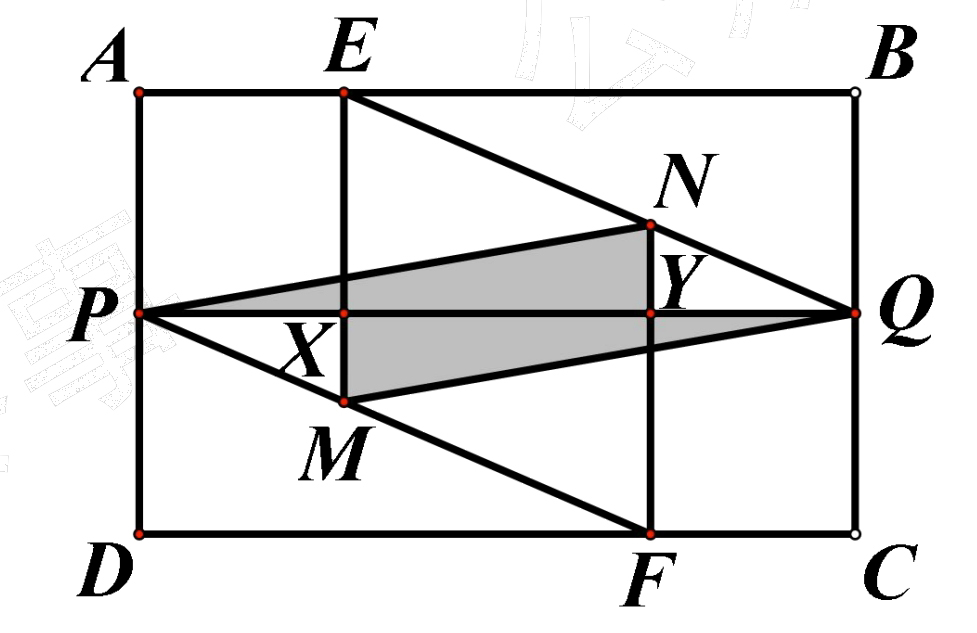
\includegraphics[width=0.4\textwidth]{./pics/Chapter_3/1.png}
    \end{figure}
    \vspace{1cm}
    % 17
}

\item {
    如图,边长为24的大正方形被分成了五个周长相等的长方形,那么阴影长方形的面积是 \underline{\hbox to 20mm{}}.
    \begin{figure}[H] 
        \centering
        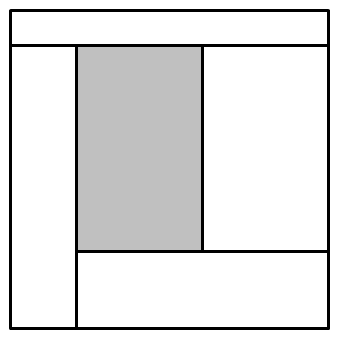
\includegraphics[width=0.2\textwidth]{./pics/Chapter_3/2.png}
    \end{figure}
    \vspace{1cm}
    % 
}

\item {
    如图,正六边形ABCDEF中,以AB为边长向内作正方形ABGH,CG与FH交于点M.\\
    (1)如果正六边形ABCDEF的边长是20,那么三角形AFH的面积是\underline{\hbox to 20mm{}}.\\
    (2)如果正六边形ABCDEF的面积是24,那么阴影部分面积之和是\underline{\hbox to 20mm{}}.
    \begin{figure}[H] 
        \centering
        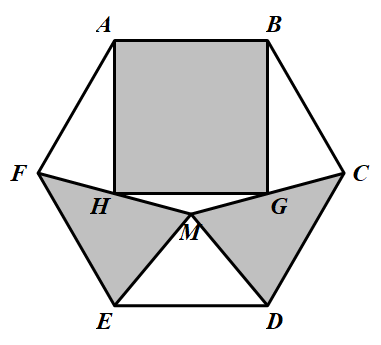
\includegraphics[width=0.4\textwidth]{./pics/Chapter_3/3.png}
    \end{figure}
    \vspace{1cm}
    % 
}
\item {
    如图,一个大正方形被分割成了周长依次为70、80、90、100的四个小长方形;那么,其中最小的小长方形的面积是\underline{\hbox to 20mm{}}.
    \begin{figure}[H] 
        \centering
        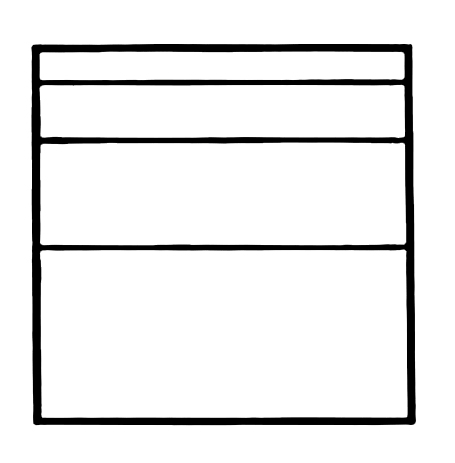
\includegraphics[width=0.2\textwidth]{./pics/Chapter_3/4.png}
    \end{figure}
    \vspace{1cm}
    % 
}

\item {
    {两个完全一样的长方形如图摆放,如果整个图形的面积是 420平方厘米,那么阴影部分的面积是\underline{\hbox to 20mm{}}平方厘米.} 
    \begin{figure}[H] 
        \centering
        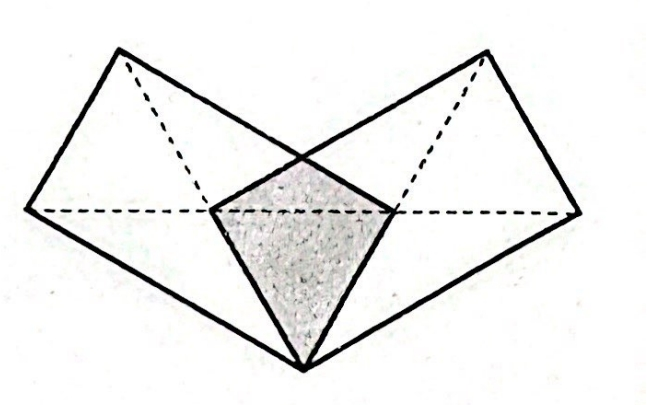
\includegraphics[width=0.4\textwidth]{./pics/Chapter_3/5.png}
    \end{figure}
    \vspace{1cm}
    % 84
}
\item {
    {在一个长方形纸片的左下角剪掉一个小长方形,
    再切成三块, 这三块恰好可以拼成一个三角形,
    若长方形的宽为12, AB的长度是CD的5倍,
    那么EC的长度为\underline{\hbox to 20mm{}}.} 
    \begin{figure}[H] 
        \centering
        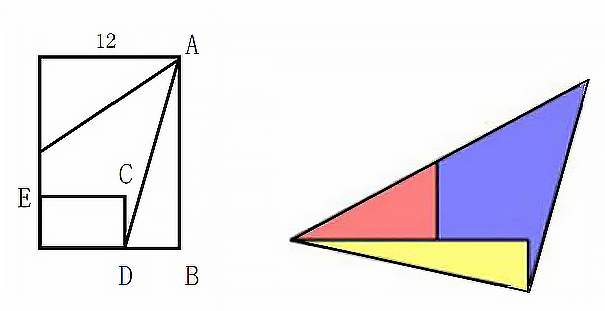
\includegraphics[width=0.6\textwidth]{./pics/Chapter_3/6.png}
    \end{figure}
    \vspace{1cm}
    % 
}

\item {
    {如图所示,一个正五边形与两个正六边形相邻,它们的边长相等。则$\angle ABC = $\underline{\hbox to 20mm{}}.} 
    \begin{figure}[H] 
        \centering
        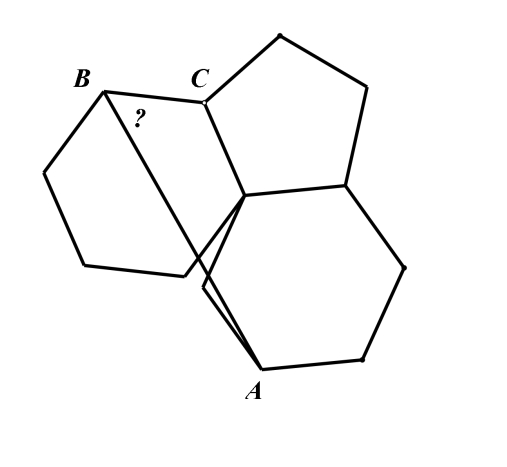
\includegraphics[width=0.4\textwidth]{./pics/Chapter_3/7.png}
    \end{figure}
    \vspace{1cm}
    % 华杯202103
}
\item {
    {如图,三角形 ABC和三角形 ADE是 $\angle A=90\degree$ 的等腰直角三角形,点 M 是 BC 的中点。已知$AB=AC=DF=FM=EG=GM$, $\angle FDE = \angle GED=9\degree$ 且点F和点G在三角形ADE以外. 问$\angle FMG$ 的度数是( )度.} 
    \begin{figure}[H] 
        \centering
        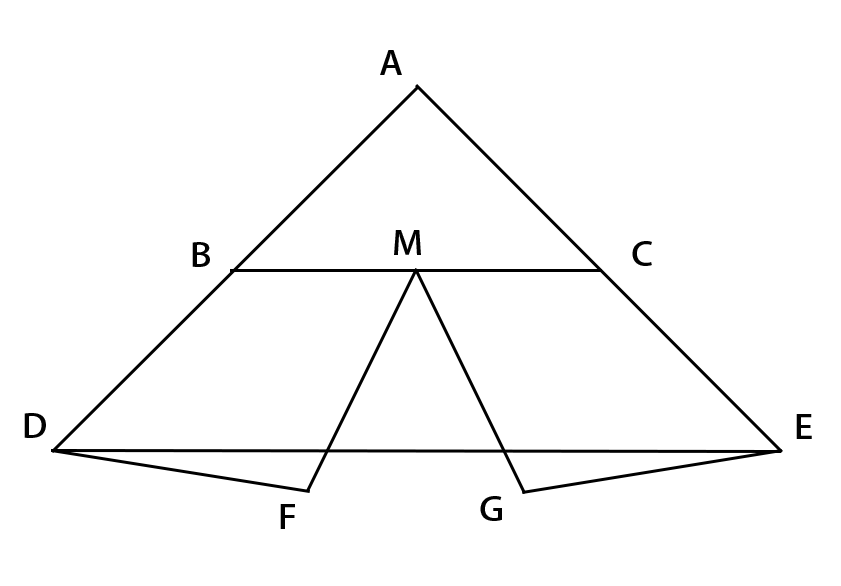
\includegraphics[width=0.4\textwidth]{./pics/Chapter_3/8.png}
    \end{figure}
    \vspace{1cm}
    % 华数真题2021-2023(小中组).pdf, 2022.2.19线上小中组解析1.pdf; 54
}

\item {
    {在下图中,$\angle 1 + \angle 2 + \angle 3 + \angle 4 - \angle 5=$ \underline{\hbox to 20mm{}} $\degree$.} 
    \begin{figure}[H] 
        \centering
        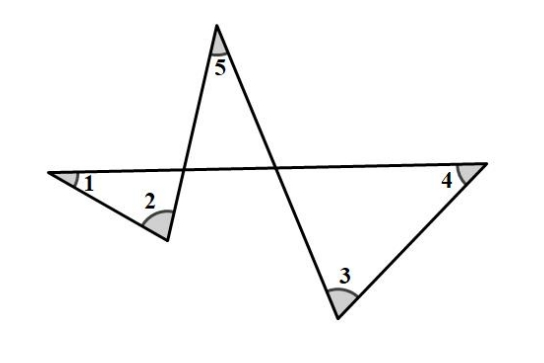
\includegraphics[width=0.4\textwidth]{./pics/Chapter_3/9.png}
    \end{figure}
    \vspace{1cm}
    % 华数真题2021-2023(小中组).pdf
}
\item {
    {如图所示,一个正方形纸片ABCD沿对角线BD剪成两个三角形.第一步操作,将三角形ABD竖直向下平移3厘米至三角形EFG;第二步操作,将三角形EFG竖直向下再平移5厘米至三角形HIJ.第一步操作后两张纸片重叠的面积与第二步操作后两张纸片重叠的面积相等,那么这个正方形纸片ABCD的面积是 \underline{\hbox to 10mm{}} 平方厘米.} 
    \begin{figure}[H] 
        \centering
        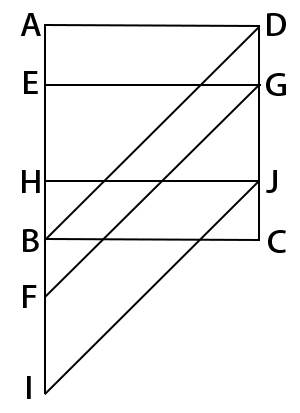
\includegraphics[width=0.2\textwidth]{./pics/Chapter_3/10.png}
    \end{figure}
    \vspace{1cm}
    % 2018年第二十三届“华罗庚金杯”少年数学邀请赛初赛试卷(小中组).doc; 121
}

\item {
    {从四边形4个内角取2个求和,共有6个和数,则大于180°的和最多有 \underline{\hbox to 20mm{}} 个.} 
    \begin{figure}[H] 
        \centering
        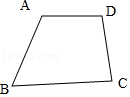
\includegraphics[width=0.2\textwidth]{./pics/Chapter_3/11.png}
    \end{figure}
    \vspace{1cm}
    % 华杯2018; 3
}
\item {
    {如图,将一个正方形硬纸片的四个角分别剪去一个等腰直角三角形,最后剩下一个长方形.正方形边长和三角形直角边长都是整数.若剪去部分的总面积为40平方厘米,则长方形的面积是 \underline{\hbox to 20mm{}} 平方厘米.} 
    \begin{figure}[H] 
        \centering
        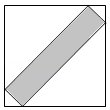
\includegraphics[width=0.2\textwidth]{./pics/Chapter_3/12.png}
    \end{figure}
    \vspace{1cm}
    % 2017年第二十二届“华罗庚金杯”少年数学邀请赛决赛试卷(小中组).doc; 24
}

\item {
    {如图所示,两个边长为6的正方形ABFE和CDEF拼成长方形ABCD.G为DE的中点.连接BG交EF于H.求图中五边形CDGHF的面积.} 
    \begin{figure}[H] 
        \centering
        
\includegraphics[width=0.4\textwidth]{./pics/Chapter_3/13.png}
    \end{figure}
    \vspace{1cm}
    % 华杯2017; 33
}
\item {
    {图中的八边形是将大长方形纸片剪去一个小长方形得到.则至少需要知道(\quad)条线段的长度,才可以计算出这个八边形的周长.} \\
    {A. 4\quad B. 3\quad C. 5\quad D. 10}
    \begin{figure}[H] 
        \centering
        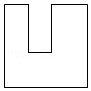
\includegraphics[width=0.2\textwidth]{./pics/Chapter_3/14.png}
    \end{figure}
    \vspace{1cm}
    % 2017年第二十二届“华罗庚金杯”少年数学邀请赛初赛试卷(小中组).doc; B
}

\item {
    {如图,在两张大小相同的大长方形纸片上,分别在角和边上各剪下一个大小相同的小正方形.若图\textcircled{2}阴影部分的周长比图\textcircled{1}阴影部分的周长多17厘米,那么剪下的小正方形周长为 \underline{\hbox to 10mm{}} 厘米.} \\
    \begin{figure}[H] 
        \centering
        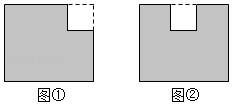
\includegraphics[width=0.4\textwidth]{./pics/Chapter_3/15.png}
    \end{figure}
    \vspace{1cm}
    % 华杯2017; 34
}

        \end{enumerate}
        \begin{enumerate}
            \section{行程问题}

\title[第4讲\quad 行程问题]{第4讲\quad 行程问题} 
\author{}
\date{}

\begin{frame}
    \titlepage
\end{frame}

\setcounter{framecounter}{0}

\begin{frame}
    \stepcounter{framecounter}
    \frametitle{习题\theframecounter}
    \vspace*{-3cm}
    \textit{一辆公共汽车和一辆小轿车同时从相距450千米的两地相向而行,公共汽车每小时行40千米,小轿车每小时行50千米,\underline{\hbox to 20mm{}}小时后两车第二次相距90千米.} 
    % 2020数学花园探秘笔试小中决赛D卷.doc; 6
\end{frame}

\begin{frame}
    \stepcounter{framecounter}
    \frametitle{习题\theframecounter}
    \vspace*{-3cm}
    \textit{小文今天和朋友约定一起看 12:00 开场的电影,出门时,发现挂钟电池没电已经停止了,她把挂钟换好电池,但没来得及调整时间,出门前挂钟显示的时间是 9:25,小文赶到电影院时,电影刚好开场.电影结束后,小文立刻返回家中,发现挂钟显示的时间是 13:55,小文赶紧把它调成正确的时间15:45.如果小文从家到电影院和从电影院返回家中花的时间是一样的,那么,电影的时长是\underline{\hbox to 10mm{}}分钟.}
    % 迎春杯四年级2022-试卷.pdf; 180
\end{frame}

\begin{frame}
    \stepcounter{framecounter}
    \frametitle{习题\theframecounter}
    \vspace*{-1cm}
    \textit{一条圆形跑道长 600 米,因铺设水管,其中跑道上 AB 一段被挖开,形成一个大坑。AB的跑道长度为 150 米。 有一机器人放在跑道上循环行走, 前进的步长(跑道弧长)为 d米,可调整步长 d的大小,但调后不再改变,并且 d小于 600 米.请设计出两种(d 的不同长度)方案,使得机器人不断循环,并且永远不会落入坑里(碰到 A或 B也算落入坑里)每种方案包括:\\
    (1)步长d的值(不同方案的d的值)。\\
    (2)机器人的出发点.}
    % 方案一:作一弧长 300米,该弧包含 AB,(4,B不在弧的端点上).机器人从该段弧的端点出发,d=300
    % 方案二:作一弧长 200 米,该弧包含 AB,(A,B不在弧的端点上).机器人从该段弧的端点出发,d=200
    % 方案三:作一弧长 400米,该弧的一半部分包含 AB,(4,B不在弧的端点与中点上).机器人从该段弧的端点出发,d=200.
    % 2021“华数之星”复评(初级)参考答案及评阅标准.pdf
\end{frame}

\begin{frame}
    \stepcounter{framecounter}
    \frametitle{习题\theframecounter}
    \vspace*{-3cm}
    \textit{哥哥和弟弟两人同时从家出发去 2000米外的学校上学,哥哥每分钟走 60米,弟弟每分钟走 50 米,走了 10 分钟后,哥哥发现忘记带数学错题本,就以每分钟 100 米的速度跑回家,回到家后,哥哥用了2分钟找到了错题本,然后以每分钟 150 米的速度往学校跑.从哥哥第二次从家出发开始计算,经过\underline{\hbox to 10mm{}}分钟后,哥哥能追上弟弟.}
    % 2020华数之星初赛-三四年级真题.pdf; 9
\end{frame}

\begin{frame}
    \stepcounter{framecounter}
    \frametitle{习题\theframecounter}
    \vspace*{-3cm}
    \textit{甲、乙两车分别从A,B两地同时出发,相向而行,3小时后相遇,甲掉头返回A地,乙继续前行.甲到达A地后掉头往B行驶,半小时后和乙相遇.那么乙从A到B共需\underline{\hbox to 10mm{}}小时.}
    % 2011华, 7.2
\end{frame}

% \begin{frame}
%     \stepcounter{framecounter}
%     \frametitle{习题\theframecounter}
%     \vspace*{-3cm}
%     \textit{甲、乙两车分别从A,B两地同时出发,相向而行,3小时后相遇,甲掉头返回A地,乙继续前行.甲到达A地后掉头往B行驶,半小时后和乙相遇.那么乙从A到B共需\underline{\hbox to 10mm{}}小时.}
%     % 2011华, 7.2
% \end{frame}

\begin{frame}
    \stepcounter{framecounter}
    \frametitle{习题\theframecounter}
    \vspace*{-3cm}
    \textit{一个车队以4米/秒的速度缓慢通过一座长298米的大桥,共用115秒,已知每辆车长6米,相临两车间隔20米,则这个车队一共有 \underline{\hbox to 10mm{}} 辆车.}
    % 2012华, 7
\end{frame}

\begin{frame}
    \stepcounter{framecounter}
    \frametitle{习题\theframecounter}
    \vspace*{-3cm}
    \textit{四百米比赛进入冲刺阶段,甲在乙前面30米,丙在丁后面60米,乙在丙前面20米.这时,跑在前面的两位同学相差 \underline{\hbox to 10mm{}} 米.}
    % 2012华, 10
\end{frame}

\begin{frame}
    \stepcounter{framecounter}
    \frametitle{习题\theframecounter}
    \vspace*{-3cm}
    \textit{里山镇到省城的高速路全长189千米,途径县城.县城离里山镇54千米.早上8:30一辆客车从里山镇开往县城,9:15到达.停留15分钟后开往省城,午前11:00能够到达.另有一辆客车于当日早上9:00从省城径直开往里山镇.每小时行驶60千米.两车相遇时,省城开往里山镇的客车行驶了 \underline{\hbox to 10mm{}} 分钟.}
    % 2012华, 72
\end{frame}

\begin{frame}
    \stepcounter{framecounter}
    \frametitle{习题\theframecounter}
    \vspace*{-3cm}
    \textit{一艘轮船,从上游A地开往下游B地,需要1小时,原路返程时,将船速提高到原来的2倍,也需要1小时.那么,如果游轮从A地出发时也采用2倍船速,需要  \underline{\hbox to 10mm{}} 分钟可以到达B地.}
    % 2014华, 36
\end{frame}

\begin{frame}
    \stepcounter{framecounter}
    \frametitle{习题\theframecounter}
    \vspace*{-3cm}
    \textit{一条河上有A,B两个码头,A在上游,B在下游.甲、乙两人分别从A,B同时出发,划船相向而行,4小时后相遇.如果甲、乙两人分别从A,B同时出发,划船同向而行,乙16小时后追上甲.已知甲在静水中划船的速度为每小时6千米,则乙在静水中划船每小时行驶\underline{\hbox to 10mm{}}千米.}
    % 2015华, 10
\end{frame}

\begin{frame}
    \stepcounter{framecounter}
    \frametitle{习题\theframecounter}
    \vspace*{-3cm}
    \textit{甲、乙两人在一条长120米的直路上来回跑,甲的速度是5米/秒,乙的速度是3米/秒,若他们同时从同一端出发跑了15分钟,则他们在这段时间内共迎面相遇 \underline{\hbox to 10mm{}} 次(端点除外).}
    % 2015华, 23
\end{frame}

\begin{frame}
    \stepcounter{framecounter}
    \frametitle{习题\theframecounter}
    \vspace*{-3cm}
    \textit{甲、乙两车分别从A,B两地同时出发,相向匀速行进,在距A地 60 千米处相遇.相遇后,两车继续行进,分别到达B,A后,立即原路返回,在距B地50 千米处再次相遇.则A,B两地的路程是\underline{\hbox to 10mm{}}千米.}
    % 2016华, 130
\end{frame}

\begin{frame}
    \stepcounter{framecounter}
    \frametitle{习题\theframecounter}
    \vspace*{-3cm}
    \textit{猎豹跑一步长为2米,狐狸跑一步长为1米.猎豹跑2步的时间狐狸跑3步.猎豹距离狐狸30米,则猎豹跑动\underline{\hbox to 10mm{}}米可追上狐狸.}
    % 2017华, 120
\end{frame}

        \end{enumerate}
        \begin{enumerate}
            \section{幂的运算}

\item {
    若$a,b$是正整数,且满足 $2^a + 2^a + 2^a + 2^a = 2^b\cdot 2^b\cdot 2^b\cdot 2^b\cdot$,则 $a$与$b$ 的关系是?\\
    \ifshowSolution
    \fangsong\zihao{4}
    \\
    思路: 

    解答:
    \else
        \\ \\ \\
    \fi
}

\item {
    $\bigstar\bigstar\bigstar\bigstar$
    (用科学记数法)一个正方体集装箱的棱长为 $0. 8 \rm{m}$. \\
    % (1) 这个集装箱的体积是多少?(用科学记数法)\\
    (2) 若有一个小立方块的棱长为$2\times 10^{-3} $ m, 则需要多少个这样的小立方块才能将集装箱装满?
    \ifshowSolution
    \fangsong\zihao{4}
    \\
    思路: 问题(2)注意简便运算. 

    解答:
    \begin{align*}
        \frac{0. 8^3} {(2\times 10^{-3})^3} &= \frac{0. 8^3} {8\times 10^{-9}}\\
        &= \frac{0. 064} {\frac{1}{10^9}}\\
        &= 0. 064\times 10^9\\
        &= 6. 4\times 10^{-2}\times 10^9\\
        &= 6. 4\times 10^7\\
    \end{align*}
    \else
        \\ \\ \\
    \fi
}

\begin{comment}
\item {
    当 $ x=7, y=-\frac{1}{7}$ 时, 求 $x^{4n+1}\cdot y^{4n+2}$ ($n$为整数)的值. 
    \ifshowSolution
        \fangsong\zihao{4}
        \\
        思路: 观察到$xy=-1$, 让将$x$和$y$凑成一对, 相乘. 直接将$x, y$的值代入表达式中进行计算. 

        解答: 
        \begin{align*}
            \mbox{原式} &= 7^{4n+1}\cdot \left(-\frac{1}{7}\right) ^{4n+2}\\
            &= [7\times(-\frac{1}{7})]^{4n+1} \cdot(-\frac{1}{7})\\
            &= (-1)^{4n+1} \cdot(-\frac{1}{7})\\
            &= \frac{1}{7}. 
        \end{align*}
    \else
        \\ \\ \\
    \fi
}

\item {
    已知$ m=8^9, n=9^8 $, 用含$m, n$的式子表示 $72^{72}$. 
    \ifshowSolution
        \fangsong\zihao{4}
        \\
        思路: 观察到$72=8\times 9$, 将原式中的72分解, 凑出$m, n$. 
        
        解答: 
        \begin{align*}
            \mbox{原式} &= (8\times 9)^{72}\\
            &= 8^{72}\times 9^{72}\\
            &= (8^9)^8\times (9^8)^9\\
            &= m^8 n^9. 
        \end{align*}
    \else
        \\ \\ \\
    \fi
}

\item {
    已知$x-y=k$, 求$(3x-3y)^3. $
    \ifshowSolution
        \fangsong\zihao{4}
        \\
        解答: 
        \begin{align*}
            \mbox{原式} &= [3(x-y)]^3\\
            &= 27(x-y)^3\\
            &= 27k^3. 
        \end{align*}
    \else
        \\ \\ \\
    \fi
}

\item {
    若$(a^nb^mb)^3 = a^9 b^{15}$, 求$2^{m+n}$. 
    \ifshowSolution
        \fangsong\zihao{4}
        \\
        思路: 先将左边化简, 再与右边比较, 解出$m, n$. 
        
        解答: 
        \begin{align*}
            (a^nb^{m+1})^3 &= a^9b^{15}\\
            a^{3n}b^{3m+3} &= a^9b^{15}
        \end{align*}
        $\therefore 3n=9, 3m+3=15$\\
        $\therefore n=3, m=4$
        \begin{align*}
            2^{m+n} &= 2^7\\
            &= 128. 
        \end{align*}
    \else
        \\ \\ \\
    \fi
}

    \item {
        化简: $(-a-b)^{2n}$ ($n$为整数). 
    }
    \\ \\ \\
    \item {
        化简: $(-a-b)^{2n+1}$ ($n$为整数). 
    }
    \\ \\ \\

    \item {
        (用科学计数法表示)已知 1 nm = 0. 000000001 m, 则 15 nm 等于多少 m?
        \ifshowSolution
        \fangsong\zihao{4}
        \\
        解答: 

        \textcircled{1} 写出换算关系
        \begin{align*}
            1 \rm{nm} &= 10^{-9} \rm{m}
        \end{align*}
        \textcircled{2} 两边同时乘15
        \begin{align*}
            15 \rm{nm} &= 15 \times 10^{-9} \rm{m}\\
            &= 1. 5\times 10^{-8} \rm{m}. 
        \end{align*}
        \fi
    }
    \\ \\ \\

    \item {
        (用科学计数法表示)肥皂泡表面厚度大约是 0. 0007 mm, 换算成以米为单位是多少?
    \ifshowSolution
    \fangsong\zihao{4}
    \\
    解答: 

    \textcircled{1} 写出换算关系
    \begin{align*}
        1 \rm{mm} &= 10^{-3} \rm{m}
    \end{align*}
    \textcircled{2} 两边同时乘0. 0007
    \begin{align*}
        0. 0007 \rm{mm} &= 0. 0007 \times 10^{-3} \rm{m}\\
        &= 7\times 10^{-7} \rm{m}. 
    \end{align*}
    \fi
    }
    \\ \\ \\

\item {
    (用科学计数法表示)已知 $0. 25 \upmu$m $ = 2. 5\times 10^{-7}$m, 那么 1 m 等于多少$\upmu$m?
    \ifshowSolution
        \fangsong\zihao{4}
        \\
        思路: 将题中给出的换算关系两边同时除以 $2. 5\times 10^{-7}$, 右边就出现了 1m. 

        解答: 
        \begin{align*}
            \frac{0. 25}{2. 5\times 10^{-7}} \rm{\upmu m} &= 1\rm{m}\\
            \frac{2. 5\times 0. 1}{2. 5\times \frac{1}{10^7}} \rm{\upmu m} &= 1\rm{m}\\
            0. 1\times 10^7 \rm{\upmu m} &= 1\rm{m}\\
            10^6 \rm{\upmu m} &= 1\rm{m}\\
            1\rm{m} &= 10^6 \rm{\upmu m}. 
        \end{align*}
    \else
        \\ \\ \\
    \fi
}

    \item {
        若多项式$ 9x^2 - mx+16$是一个完全平方式, 则 $m$的值是多少?
    }
    \\ \\ \\

\item {
    已知$a^2+b^2=8, a-b=3$, 求$ab$的值. 
    \ifshowSolution
        \fangsong\zihao{4}
        \\
        思路: 看到$a^2+b^2, a-b, ab$, 应该想到完全平方公式. 
    \else
        \\ \\ \\
    \fi
}

    \item {
        若$x^2+mx+9$是完全平方式, 求常数$m$的值. 
    }
    \\ \\ \\

    \item {
        若$x+y=2$, 求代数式$x^2-y^2+4y$的值. 
    }
    \\ \\ \\

\item {
    (注意: 除号使用分数形式) 已知$10^{-m}=a, 10^{-n}=b$($m, n$是整数), 求$10^{2m-3n}$的值(用含有$a, b$的代数式表示). 
    \\ \\ \\
}

\item {
    已知$2^x=3, 2^y=6, 2^z=12$, 判断下列有关$x, y, z$的数量关系式的对错. \\
    (1) $x+z=2y$\\
    (2) $x+y+3=2z$\\
    (3) $4x=z$\\
    (4) $x+1=y$
    \\ \\
}

\item {
    计算: $ (\frac{1}{2})^{-1} + \lvert 2-\pi \rvert $
    \ifshowSolution
    \fangsong\zihao{4}
    \\
    思路: 去绝对值符号, 运算到底. 

    解答: 
    \begin{align*}
        \mbox{原式} &= 2 + \pi - 2\\
        &= \pi. 
    \end{align*}
    \else
        \\ \\ \\
    \fi
}

\item {
    已知$(x+2)^{x+5}=1$, 求$x$. 
    \\ \\ \\
}

    \item {
        (把 $\frac{1}{27}$ 化为以3为底的幂) 若$3^{x-1}=\frac{1}{27}$, 求$x$. 
        \\ \\ \\
    }
    
\item {
    (注意: 除号使用分数形式) 已知$a^{2n}=3, a^{3m}=5$, 求$a^{6n-9m}$. 
    \ifshowSolution
    \fangsong\zihao{4}
    \\
    思路: 将$a^{6n-9m}$凑出$a^{2n}, a^{3m}$, 直接代入计算. 结果使用分数形式即可. 

    解答: 
    \begin{align*}
        a^{6n-9m} &= \frac{a^{6n}}{a^{9m}}\\
        &= \frac{(a^{2n})^3} {(a^{3m})^3}\\
        &= \frac{3^3} {5^3}\\
        &= \frac{27} {125}. 
    \end{align*}
    \else
        \\ \\ \\
    \fi
}

    \item {
        已知$3\cdot2^x + 2^{x+1}=40$, 求$x$. 
        \ifshowSolution
        \fangsong\zihao{4}
        \\
        思路: 将左边的2个$2^{x}$整理到一起. 
    
        解答: 
        \begin{align*}
            3\cdot2^x + 2^{x+1} &= 40\\
            3\cdot2^x + 2\cdot 2^{x} &= 40\\
            5\cdot2^x &= 40\\
            2^x &= 8\\
            \therefore x = 3. 
        \end{align*}
        \else
            \\ \\ \\
        \fi
    }
\end{comment}
        \end{enumerate}
    \end{sloppy}
\end{document}
